\section{Design Pattern}
\subsection{Design Pattern Architetturali}

\subsubsection{MVC - Model View Controller}

\begin{figure}[h]
\begin{center}
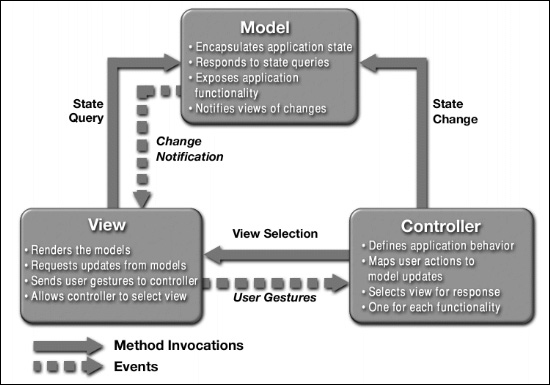
\includegraphics[scale=0.4]{img/MVC.jpg}
\caption{Diagramma del design pattern MVC}
\end{center}
\end{figure}

\begin{itemize}
\item \textbf{Descrizione:} Il design pattern$_G$ MVC permette un disaccoppiamento totale della View dalle logiche di manipolazione del Modello tramite l’introduzione di un componente, il Controller, che funga da intermediario e da coordinatore in risposta alle interazioni con l’utente. Si individuano tre componenti:

\begin{itemize}
\item Model: dati di business e regole di accesso;
\item View: rappresentazione grafica. Visualizza i dati contenuti nel model e raccoglie gli input dell’utente;
\item Controller: reazioni della UI agli input utente. Interagisce con il model in base ai comandi dell'utente (attraverso la View);
\end{itemize}

\item \textbf{Motivazione:}  Lo scopo di molte applicazioni è quello di recuperare dati e visualizzarli in maniera opportuna a seconda delle esigenze degli utenti. Poiché il flusso chiave di informazione avviene tra il dispositivo su cui sono memorizzati i dati e l'interfaccia utente, si è portati a legare insieme queste due parti per ridurre la quantità di codice e migliorare le performance dell'applicazione. 
Questo approccio, apparentemente naturale, presenta alcuni problemi significativi; uno di questi è che l'interfaccia utente tende a cambiare più in fretta rispetto al sistema di memorizzazione dei dati. 
C'è la necessità, quindi, di rendere modulari le funzionalità dell'interfaccia utente in maniera tale da poter facilmente modificare le singole parti. 
L'intento del pattern MVC è di disaccoppiare il più possibile tra loro le parti dell'applicazione adibite al controllo, all'accesso ai dati e alla presentazione, apportando diversi vantaggi:

\begin{itemize}
\item indipendenza tra i business data (model) la logica di presentazione (view) e quella di controllo (controller);
\item separazione dei ruoli e delle relative interfacce;
\item viste diverse per il medesimo model;
\item semplice il supporto per nuove tipologie di client: bisogna scrivere la vista ed il controller appropriati riutilizzando il model esistente.
\end{itemize}

\item \textbf{Applicablità:} Il pattern MVC può essere utilizzato nei seguenti casi:

\begin{itemize}
\item Quando si vuole trattare un gruppo di oggetti come un oggetto singolo;
\item Quando si vuole disaccoppiare View e Model instaurando un protocollo di sottoscrizione e notifica tra loro;
\item Quando si vogliono agganciare più View a un Model per fornire più rappresentazioni del Model stesso.
\end{itemize}

\end{itemize}

\subsubsection{MVVM - Model View VievModel}

\begin{figure}[h]
\begin{center}
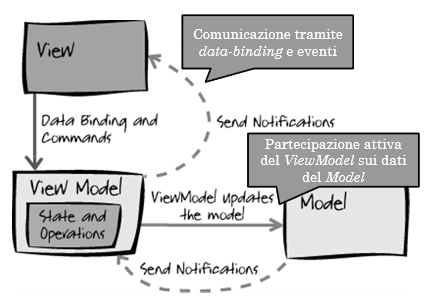
\includegraphics[scale=0.5]{img/MVVM.png}
\caption{Diagramma del design pattern MVVM}
\end{center}
\end{figure}

\begin{itemize}
\item \textbf{Descrizione:} Il design pattern$_G$ MVVM è una variante del pattern MVC che propone un ruolo più attivo della View, la quale è in grado di gestire eventi, eseguire operazioni ed effettuare il data-binding. In questo contesto, quindi, alcune delle funzionalità del Controller vengono inglobate nella View, la quale si appoggia su un’estensione del Model: il ViewModel. Come per il pattern MVC, anche quì si individuano tre componenti:

\begin{itemize}
\item Model: dati di business e regole di accesso;
\item View: rappresentazione grafica. Visualizza i dati contenuti nel model e raccoglie gli input dell’utente;
\item ViewModel: Model esteso con funzionalità per la manipolazione dei dati e per l’interazione con la View.
\end{itemize}

\item \textbf{Motivazione:}  Il cuore del funzionamento di questo pattern è la creazione di un componente (ViewModel) che rappresenta, in modo astratto, tutte le informazioni e i comportamenti della corrispondente View; quest'ultima si limita a visualizzare graficamente quanto esposto dal ViewModel, a riflettere i propri cambi di stato nel ViewModel stesso oppure ad attivare suoi comportamenti. 
L'uso di questo pattern richiede la presenza, nella tecnologia di UI, di un'ottimo meccanismo di data-binding (tipicamente bidirezionale) o, in alternativa, di un strato di sincronizzazione fra la View e il ViewModel.
E' compito del ViewModel, però, offrire alla View una "superficie esterna" il più possibile ben fruibile, in modo che la sincronizzazione dello stato possa essere fatta senza introdurre logiche decisionali che rendano necessario un test specifico.

\item \textbf{Applicablità:} Il pattern MVVM può essere utilizzato nei seguenti casi:

\begin{itemize}
\item Quando si vuole trattare un gruppo di oggetti come un oggetto singolo;
\item Quando si vuole disaccoppiare View e Model instaurando un protocollo di sottoscrizione e notifica tra loro;
\end{itemize}

\end{itemize}

\subsubsection{Dependecy Injection}

\begin{figure}[h]
\begin{center}
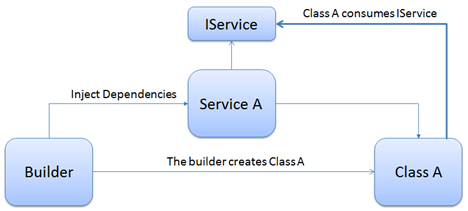
\includegraphics[scale=0.8]{img/dependency.png}
\caption{Diagramma del design pattern Dependency Injection}
\end{center}
\end{figure}

\begin{itemize}
\item \textbf{Descrizione:} Il design pattern$_G$ Dependecy Injection ha lo scopo di semplificare lo sviluppo e migliorare la testabilità del software, permettendo la separazione del comportamento di una componente dalla risoluzione delle sue dipendenze;
Il pattern Dependency Injection coinvolge almeno tre elementi:

\begin{itemize}
\item una componente \textit{dipendente};
\item la dichiarazione delle \textit{dipendenze} del componente, definite come \textit{interface contracts};
\item un \textit{injector} (chiamato anche \textit{provider} o \textit{container}) che crea, a richiesta, le istanze delle classi che implementano delle \textit{dependency interfaces}.
\end{itemize}

\item \textbf{Motivazione:} Il collegamento di due o più componenti in modo esplicito ne aumenta l'accoppiamento, causando una scarsa manutenibilità del software e complicando le fasi di unit testing.
Inoltre un componente soggetto a dipendenze risulta meno predisposto al riutilizzo dello stesso.
La dependency injection prende il controllo su tutti gli aspetti di creazione degli oggetti e delle loro dipendenze. Normalmente, senza l'utilizzo di questa tecnica, se un oggetto necessita di accedere ad un particolare servizio, l'oggetto stesso si prende la responsabilità di gestirlo, o avendo un diretto riferimento al servizio, o individuandolo con un Service Locator che gli restituisce un riferimento ad una specifica implementazione del servizio. 
Con l'utilizzo della dependency injection, l'oggetto ha in sé solamente una proprietà che può ospitare un riferimento a quel servizio e, quando l'oggetto viene istanziato, un riferimento ad una implementazione di questo servizio gli viene iniettata dal framework$_G$ esterno, senza che il programmatore che crea l'oggetto sappia nulla sul posizionamento del servizio o altri dettagli dello stesso.
\item \textbf{Applicablità:} Il pattern Dependency Injection può essere utilizzato nei seguenti casi:

\begin{itemize}
\item Quando si ha la necessità di collegare più componenti cercando di minimizzare il livello di accoppiamento;
\item Quando si lavora su progetti basati sul Test Driven.
\end{itemize}

\end{itemize}

\subsection{Design Pattern Creazionali}

\subsubsection{Factory Method}

\begin{figure}[h]
\begin{center}
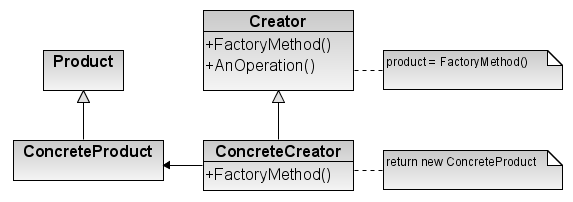
\includegraphics[scale=0.4]{img/Factory.png}
\caption{Diagramma del design pattern Factory Method}
\end{center}
\end{figure}

\begin{itemize}
\item \textbf{Descrizione:} il design pattern$_G$ Factory Method indirizza il problema della creazione di oggetti senza specificarne l’esatta classe, fornendo un’interfaccia per creare un oggetto, ma lasciando che le sottoclassi decidano quale oggetto istanziare. Definisce un’interfaccia (Creator) per ottenere una nuova istanza di un oggetto (Product).
Delega ad una classe derivata (ConcreteCreator) la scelta di quale classe istanziare (ConcreteProduct);
\item \textbf{Motivazione:} la creazione di un oggetto può, spesso, richiedere processi complessi la cui collocazione all’interno della classe di composizione potrebbe non essere appropriata.
Esso può, inoltre, comportare duplicazione di codice, richiedere informazioni non accessibili alla classe di composizione, o non fornire un sufficiente livello di astrazione.
Il Factory Method indirizza questi problemi definendo un metodo separato per la creazione degli oggetti. Tale metodo può essere ridefinito dalle sottoclassi per definire il tipo derivato di prodotto che verrà effettivamente creato;
\item \textbf{Applicablità:} Il pattern Factory Method si puù utilizzare nei seguenti casi:

\begin{itemize}
\item Quando si desidera che la creazione di un oggetto non precluda il suo riuso senza una significativa duplicazione di codice;
\item Quando si desidera che la creazione di un oggetto non richieda l’accesso ad informazioni o risorse che non dovrebbero essere contenute nella classe di composizione;
\item Quando si desidera che la gestione del ciclo di vita degli oggetti gestiti debba essere centralizzata in modo da assicurare un comportamento consistente all’interno dell’applicazione.
\end{itemize} 

\end{itemize}

\newpage